\documentclass{article}
\usepackage[utf8]{inputenc}
\title{Verification : Homework 5}
\author{Marius Belly - Le Guilloux}
\date{November 2021}


\usepackage{stmaryrd}   %N
\usepackage{esvect}     %Vector
\usepackage{hyperref}   %hypertext link
\usepackage{graphicx}
\usepackage{amsmath}    %overset
\usepackage{amssymb}    %square
\usepackage{amsthm}     %proof
\usepackage{xcolor}     %color
\usepackage{esvect}     %Vector
\usepackage{tikz}       %draw
\usetikzlibrary{positioning}
\usetikzlibrary{automata}
\usetikzlibrary{arrows}


%%% Operator %%%
\newcommand{\norm}[1]{\left\Vert #1 \right\Vert}
\newcommand{\card}[1]{\ensuremath{\left\|#1 \right\|}}
\newcommand{\interval}[2]{\ensuremath{\llbracket #1, \; #2 \rrbracket}}
\newcommand{\set}[1]{\{ #1 \}}
\newcommand{\br}[1]{\ensuremath{\llbracket #1 \rrbracket}} %Interpretation
\newcommand{\floor}[1]{\lfloor #1 \rfloor}
\newcommand{\ceil}[1]{\lceil #1 \rceil}
\newcommand{\ol}[1]{\overline{#1}}
\newcommand{\ul}[1]{\underline{#1}}

% Shortcuts sets
\newcommand{\bb}[1]{\mathbb{#1}}
\newcommand{\mc}[1]{\mathcal{#1}} %Abrev mathcal
\newcommand{\N}{\ensuremath{\mathbb{N}}}
\newcommand{\Z}{\ensuremath{\mathbb{Z}}}
\newcommand{\Q}{\ensuremath{\mathbb{Q}}}
\newcommand{\C}{\ensuremath{\mathbb{C}}}

%%% shorcuts logic %%%
\newcommand{\G}{\Gamma} % Abreviation pour logique etc..
\newcommand{\D}{\Delta} % Abreviation pour logique
\newcommand{\T}{\mathcal{T}} %Abreviation T pour logique

\newcommand{\V}{\mathcal{V}}
\newcommand{\A}{\mathcal{A}}
\newcommand{\R}{\mathcal{R}}


\begin{document}
\maketitle
\section*{Exercise 1}

\subsection*{a)}

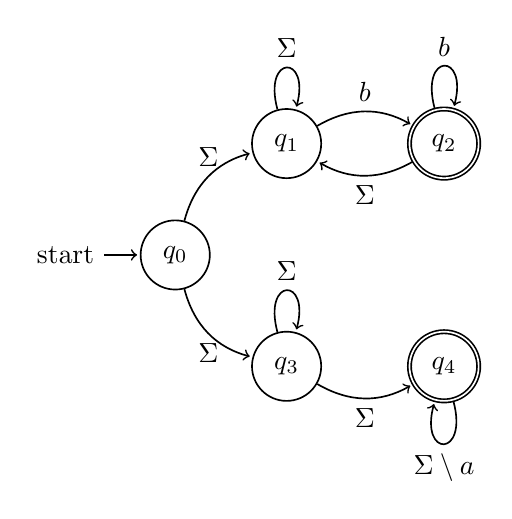
\begin{tikzpicture}[->,shorten >=1pt,auto,node distance=2cm,semithick]
\node[initial,state]   (A)                    {$q_0$};
\node[state]           (B) [above right of=A] {$q_1$};
\node[accepting,state] (C) [right of=B] 	  {$q_2$};
\node[state]           (D) [below right of=A] {$q_3$};
\node[accepting,state] (E) [right of=D] {$q_4$};

\path (A)   edge [above,bend left] node {$\Sigma$} (B)
      (B)   edge [loop above] 		node {$\Sigma$} (B)
      (B)   edge [above,bend left] node {$b$} (C)
      (C)   edge [below,bend left] node {$\Sigma$} (B)
      (C)   edge [loop above] node {$b$} (C)
      (A)   edge [below,bend right] node {$\Sigma$} (D)
      (D)   edge [loop above] 		node {$\Sigma$} (D)
      (D)   edge [below,bend right] node {$\Sigma$} (E)
      (E)   edge [loop below, below] node {$\Sigma \setminus a$} (E);
               
\end{tikzpicture}

\subsection*{b)}

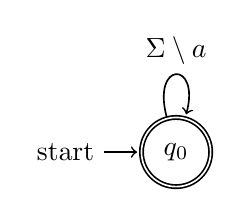
\begin{tikzpicture}[->,shorten >=1pt,auto,node distance=2cm,semithick]
\node[initial,state,accepting]   (A)  {$q_0$};

\path (A)   edge [above,loop above] node {$\Sigma \setminus a$} (A);
               
\end{tikzpicture}



\subsection*{c)}

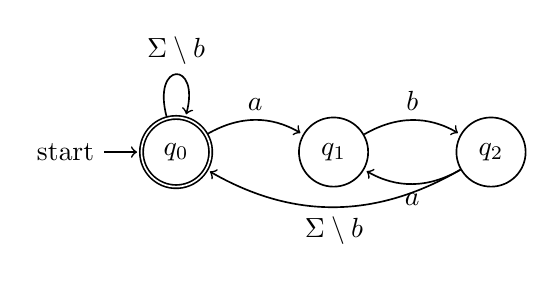
\begin{tikzpicture}[->,shorten >=1pt,auto,node distance=2cm,semithick]
\node[accepting,initial,state]   (A)                  {$q_0$};
\node[state]           			 (B) [right of=A] 	  {$q_1$};
\node[state] 					 (C) [right of=B] 	  {$q_2$};

\path (A)   edge [loop above] node {$\Sigma \setminus b$} (A)
	  (A)   edge [above,bend left] node {$a$} (B)
      (B)   edge [above,bend left] node {$b$} (C)
      (C)   edge [below,bend left] node {$\Sigma \setminus b$} (A)
      (C)   edge [below,bend left] node {$a$} (B);
               
\end{tikzpicture}

\subsection*{d)}

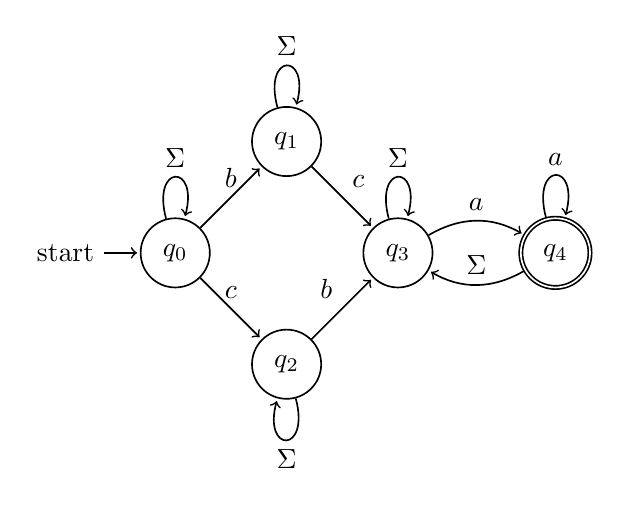
\begin{tikzpicture}[->,shorten >=1pt,auto,node distance=2cm,semithick]
\node[initial,state]   (A)                    {$q_0$};
\node[state]           (B) [above right of=A] {$q_1$};
\node[state]           (C) [below right of=A] {$q_2$};
\node[state] 		   (D) [above right of=C] {$q_3$};
\node[state,accepting] (E) [right of=D] 	  {$q_4$};


\path (A)   edge [loop above] node {$\Sigma$} (A)
      (A)   edge [above] node {$b$} (B)
      (A)   edge [above] node {$c$} (C)
      (B)   edge [loop above] node {$\Sigma$} (B)
      (B)   edge  			  node {$c$} (D)
      (C)   edge [loop below] node {$\Sigma$} (C)
      (C)   edge  			  node {$b$} (D)
	  (D)   edge [loop above] node {$\Sigma$} (D)
	  (D)   edge [above,bend left] node {$a$} (E)
	  (E)   edge [loop above] node {$a$} (E)
	  (E)   edge [above,bend left] node {$\Sigma$} (D);

\end{tikzpicture}






\section*{Exercise 2}

Let $L_i$ be recognized by a BA $\A_i = (Q_i,\Sigma,I_i,T_i,F_i)$ \newline
Let $L'_i$ be recognized by a DBA $\A'_i = (Q'_i,\Sigma,q_{init_i},T'_i,F_i)$
\subsection*{a)}

$L_1 \cap L_2$ is recognized by $\A = (Q_1 \times Q_2 \times \{1,2\},\Sigma,I_1 \times I_2 \times \{1\},T,F_1 \times Q_2 \times \{1 \})$, \newline
where $T$ is defined as follows :  \newline
$T = \underset{i \in \{1,2\}}{\bigcup} \{ ((q_1,q_2,i),a,(q'_1,q'_2,i)) \vert (q_1,a,q'_1) \in T_1,~(q_2,a,q'_2) \in T_2,~q_i \notin F_i\} \cup \newline
\{ ((q_1,q_2,1),a,(q'_1,q'_2,2)) \vert (q_1,a,q'_1) \in T_1,~(q_2,a,q'_2) \in T_2,~q_1 \in F_1\} \cup \newline
\{ ((q_1,q_2,2),a,(q'_1,q'_2,1)) \vert (q_1,a,q'_1) \in T_1,~(q_2,a,q'_2) \in T_2,~q_2 \in F_2\}$ \newline
Intuitively, this automaton runs two copies of the automata running in parallel and switches from copy $i$ to the other only when it reaches a state in $F_i$.
An accepting word would then necessarily switch infinetely many times from a copy to another, that is, reaching infinitely many times both $F_1$ and $F_2$

\subsection*{b)}

We may notice that the previous construction is a deterministic Büchi automaton if $\A_1$ and $\A_2$ are.
This observation is sufficient to prove that $L'_1 \cap L'_2$ is recognized by a DBA.

\subsection*{c)}

Let $q$ be a fresh state.\newline
$L_1 \cup \L_2$ is recognized by $\A = (\{q\} \sqcup Q_1 \sqcup Q_2,\Sigma,\{q\},T,F_1 \sqcup F_2)$, \newline
where $T = T_1 \sqcup T_2 \sqcup \{(q,a,q_1) \vert \exists q_{s_1} \in I_1 \text{ s.t } (q_{s_1},a,q_1) \in T_1\} \sqcup \newline
\{(q,a,q_2) \vert \exists q_{s_2} \in I_2 \text{ s.t } (q_{s_2},a,q_2) \in T_2\}$ \newline
Intuitively, this automaton chooses non-deterministically which automaton will actually be executed.\newline
An example of this construction may be find in Exercise 1, item a).

\subsection*{d)} 

$L'_1 \cap L'_2$ is recognized by $\A' = (Q'_1 \times Q'_2,\Sigma,(q_{init_1},q_{init_2}),T'_1 \times T'_2,F'_1 \times Q'_2 \cup Q'_1 \times F'_2)$, \newline
The construction is similar to the one used for the intersection but uses only one copy and accepts if and only if one of the two sets of targets is visited infinitely many times (by the pigeonhole principle).

\newpage


\end{document}
